\chapter{Design Methodology}
Define specs; select architecture; perform small-signal and large-signal simulations; run PSS/Pnoise or time-domain jitter; tune \(K_{VCO}\); linearize tuning; validate across PVT; finalize layout.

\section{Meta-Heuristic Optimization (Bonus)}
Apply a simple GA/PSO to choose \(L\), varactor bank size, and bias to minimize a cost combining PN@offsets, power, and tuning coverage. The flow evaluates a fast surrogate (analytical + corner multipliers) and verifies finalists with detailed simulations. Convergence typically occurs in tens of iterations; constraints enforce KVCO and range.

\begin{figure}[H]
  \centering
  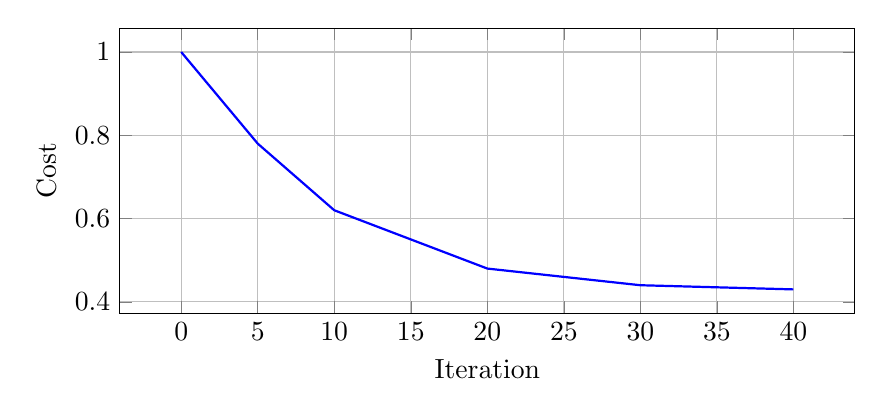
\begin{tikzpicture}
    \begin{axis}[width=0.9\linewidth, height=5.2cm, xlabel={Iteration}, ylabel={Cost}, grid=both]
      \addplot[blue, thick] table[row sep=\\]{x y \\
        0  1.00 \\
        5  0.78 \\
        10 0.62 \\
        20 0.48 \\
        30 0.44 \\
        40 0.43 \\
      };
    \end{axis}
  \end{tikzpicture}
  \caption{Illustrative convergence of a meta-heuristic cost function}
\end{figure}


